\documentclass[11pt,letterpaper]{article}
\usepackage[utf8]{inputenc}
\usepackage{amsmath,amssymb,fullpage,graphicx}
\usepackage{subfigure}
\let\hat\widehat
\let\tilde\widetilde

\begin{document}
\subsection*{Q4-a}
\noindent We may choose $D-skew = (n - 1)^{-\frac{3}{2}} \sum R_i^3$ as discrepancy statistic for both smoke and non-smoke dataset. $R_i = \frac{X_i - \bar{X}}{S}$ since variance is unknown.

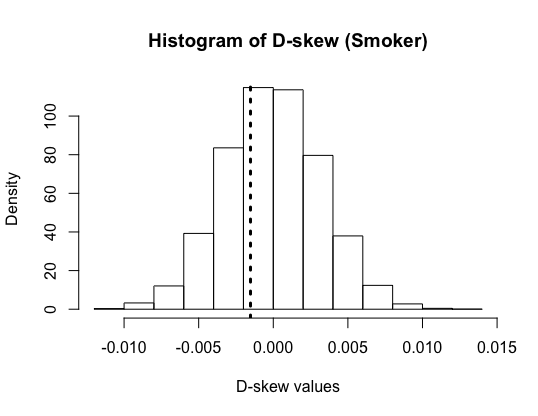
\includegraphics[scale=0.5]{q4-a-smoke.png}

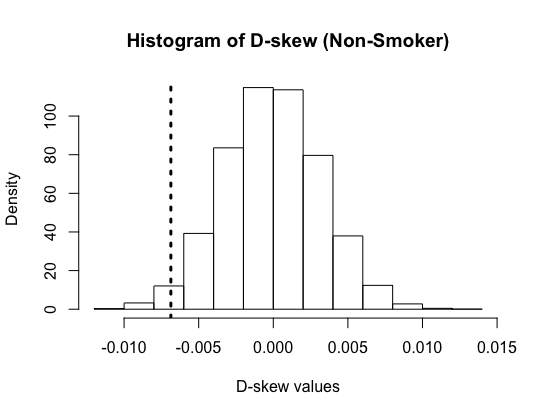
\includegraphics[scale=0.5]{q4-a-nonsmoke.png}

\noindent For non-smoker group, the discrepancy statistic is $-0.006864402$, and its p-value is $0.0332$. 

\noindent 	For smoker group, the discrepancy statistic for observed data is $-0.001527044$, and its p-value is $0.75$.\\

\noindent In smokers' group, p-value of the observed discrepancy statistic is $0.75$, which provides significant evidence that normality model might be correct.

\noindent While in non-smokers' group, p-value is $0.03$, of which under test size of $0.05$, it provides evidence to state that normality model may be incorrect for non-smoker's baby weight. 

\subsection*{q4-b}

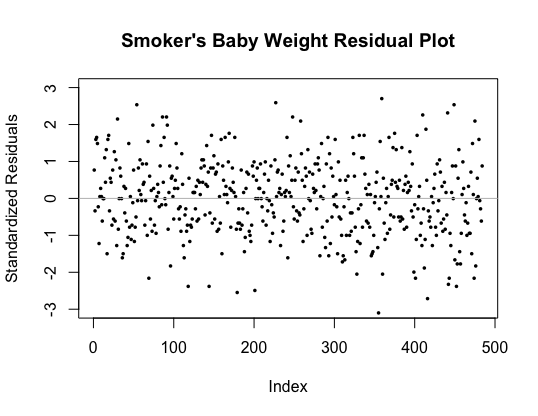
\includegraphics[scale=0.6]{q4-b-smoke.png}

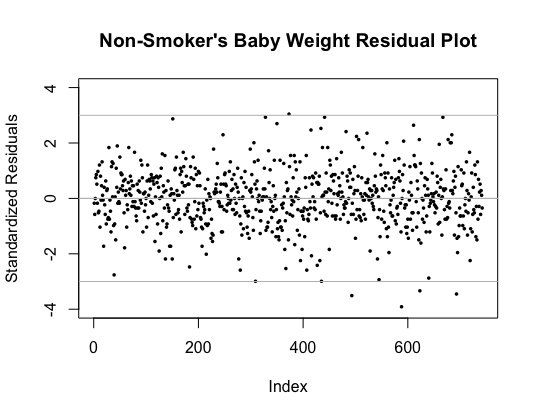
\includegraphics[scale=0.6]{q4-b-nonsmoke.png}

\noindent For both residual plot, we may perceive that data points are denser around horizontal line where residual equals zero, i.e. there are more data close to mean value than far away from it. Data points distributed above or below zero evenly, i.e. the density of data are almost symmetric around the mean value. 

\noindent Nevertheless, there are few data points in non-smokers' group have standardized residuals greater than $3$ or less than $-3$ (points themselves are 3 standard deviations away from the mean). These extreme values might make non-smokers' baby weight less likely to follow normal distribution.

\newpage
\subsection*{Q4-c}

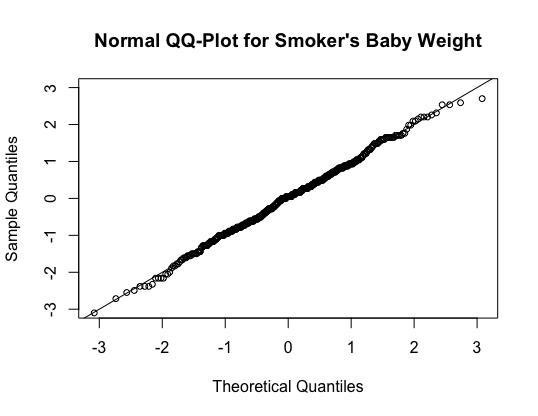
\includegraphics[scale=0.6]{q4-c-smoke.png}

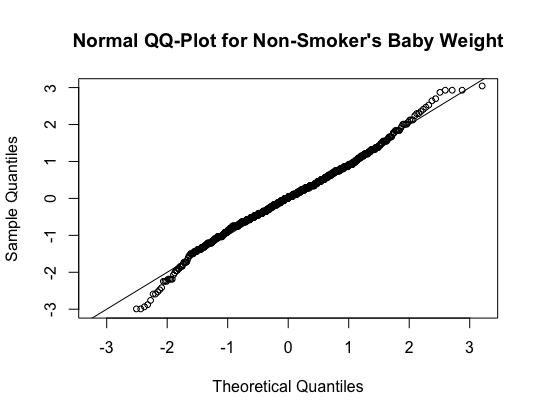
\includegraphics[scale=0.6]{q4-c-nonsmoke.png}

\noindent From the normal qq-plot of smokers' group, we can perceive that observed quantiles fit theoretical quantiles very well, which provides evidence that the sample data might follow normal distribution. \\

\noindent For non-smokers' group, observed quantiles seem not to fit theoretical quantiles at two tails, due to more lower values and higher values appeared in observed data than normal distribution. 




\end{document}